% $Id: introduction.tex 65669 2015-01-09 14:55:20Z tgershon $

\section{Detector}
\label{sec:Detector}

The \lhcb detector is a unique and specialised apparatus that has been optimised to meet the specific physics goals discussed in section \ref{sec:Introduction}, which largely involve the study of mesons and baryons containing beauty and charm quarks.  The resulting design is a single arm forward spectrometer which covers the pseudorapidity range $2 < \eta < 5$.  A schematic diagram of the detector is shown in \ref{fig:detectdiag}.This limited angular coverage is motivated by the polar angle distribution of  $b$ and $\bar{b}$ quark production peaking at small angles to the beam pipe in both the forward and backward direction, as shown in figure \ref{fig:bbarprod}.  The consequence of this angular distribution is that at 8 TeV approximately $25\%$ of $b$ or $\bar{b}$ quarks are produced within the angular acceptance of the \lhcb detector, despite the geometrical acceptance of the detector being only $~0.09$ steradians ($0.7\%$ of a full sphere).

%Luminosity
Another unique characteristic of the \lhcb detector is the lower luminosity that it operates at.  During run 1 the \atlas and \cms detectors made use of a peak luminosity of $7\times 10^{33}cm^{-2}s^{-1}$ at the start of a fill which gradually decreased over the 6-8 hour lifetime of the fill as collisions took place.  However, \lhcb ran at a lower, levelled, luminosity of $4\times 10^{32}cm^{-2}s^{-1}$.  The process of luminosity levelling (at \lhcb) involves offestting the LHC proton beams in the transverse direction to reduce the probability of interaction \cite{Follin:2014nva}. As the luminosity of the \lhc decreases over the lifetime of the fill, the beam offset at \lhcb is decreased to keep the instantaneous luminosity delivered at \lhcb constant.  The result of this lower luminosity is only a mean number of proton-proton interactions per bunch crossing of 2.5 compared to 20 as experienced by the general purpose LHC detectors.  Consequently, the radiation hardness requirements of the \lhcb detector are reduced and backgrounds from other interactions in the same bunch crossing are also significantly lower.  This lower level of background is very advantageous for rare decay searches such as \Bz \to \muon \muon.
\begin{figure}[h]
  \centering
  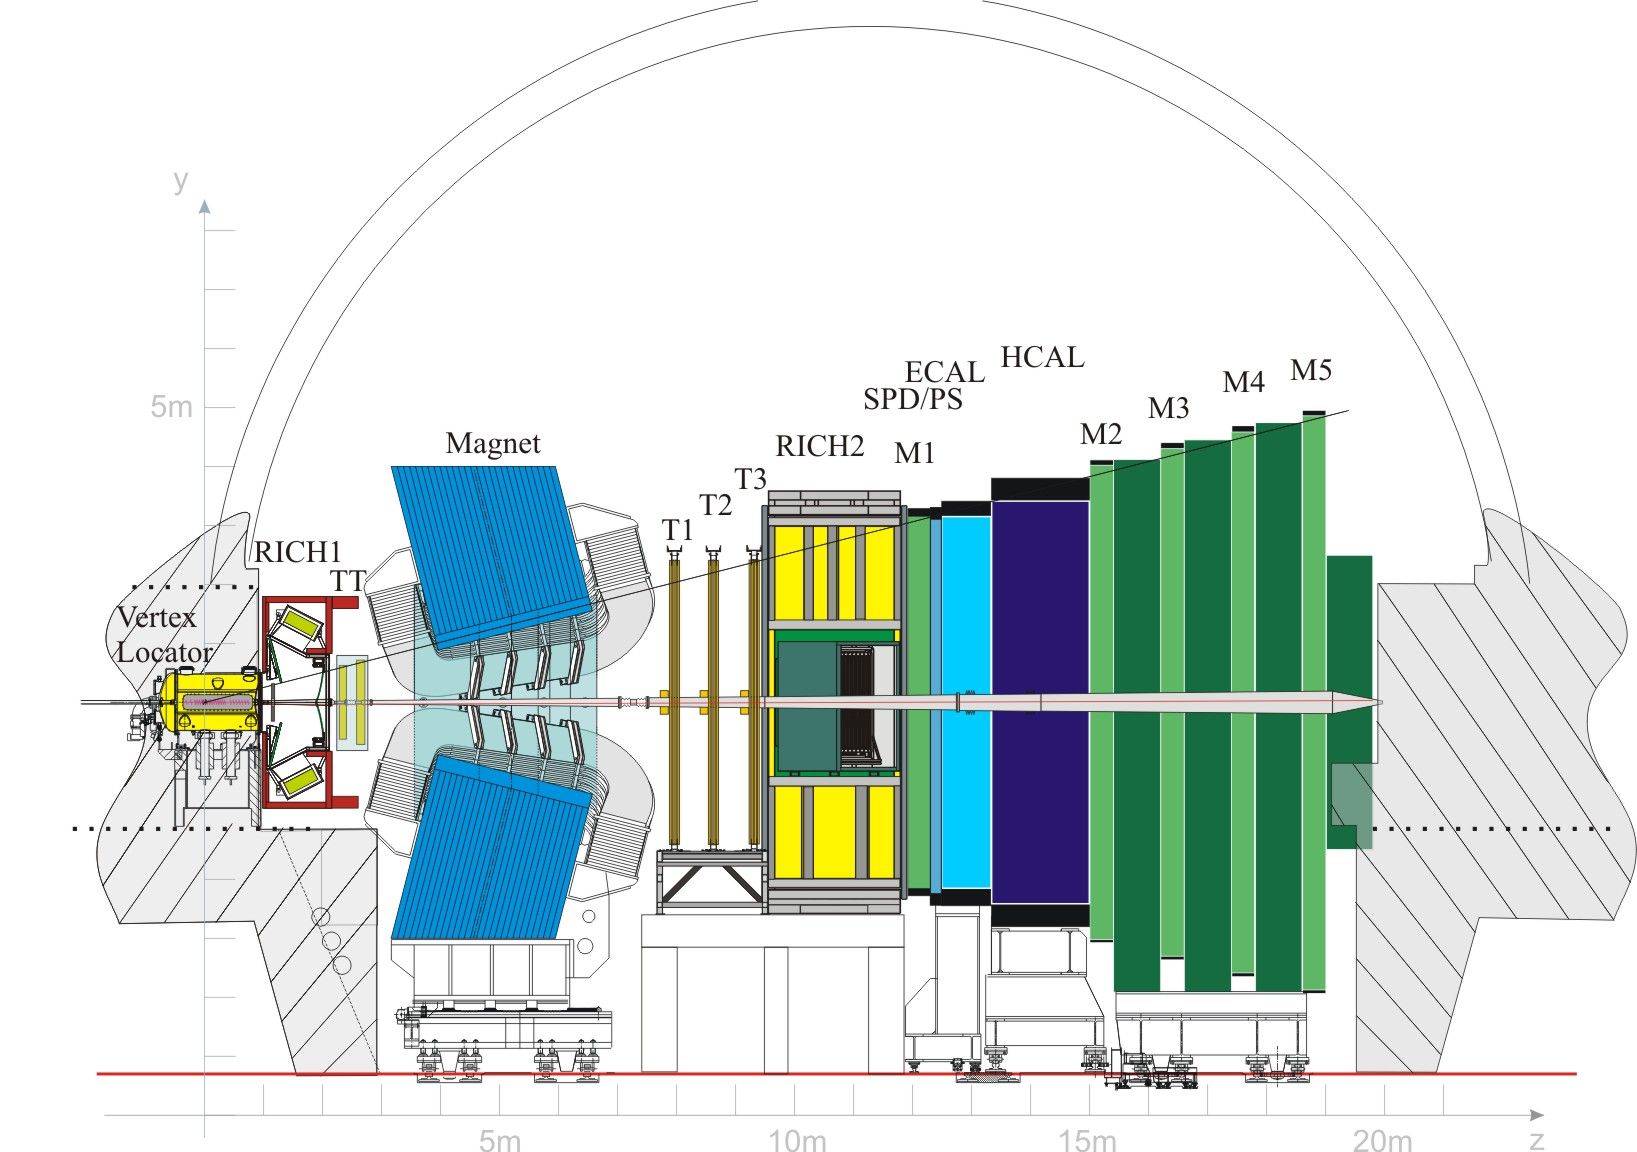
\includegraphics[width=\textwidth]{detectordiag.jpg}
  \caption{ A schematic diagram of the \lhcb detector and all its componens}
  \label{fig:detectdiag}
\end{figure}
\begin{figure}[h]
  \centering
  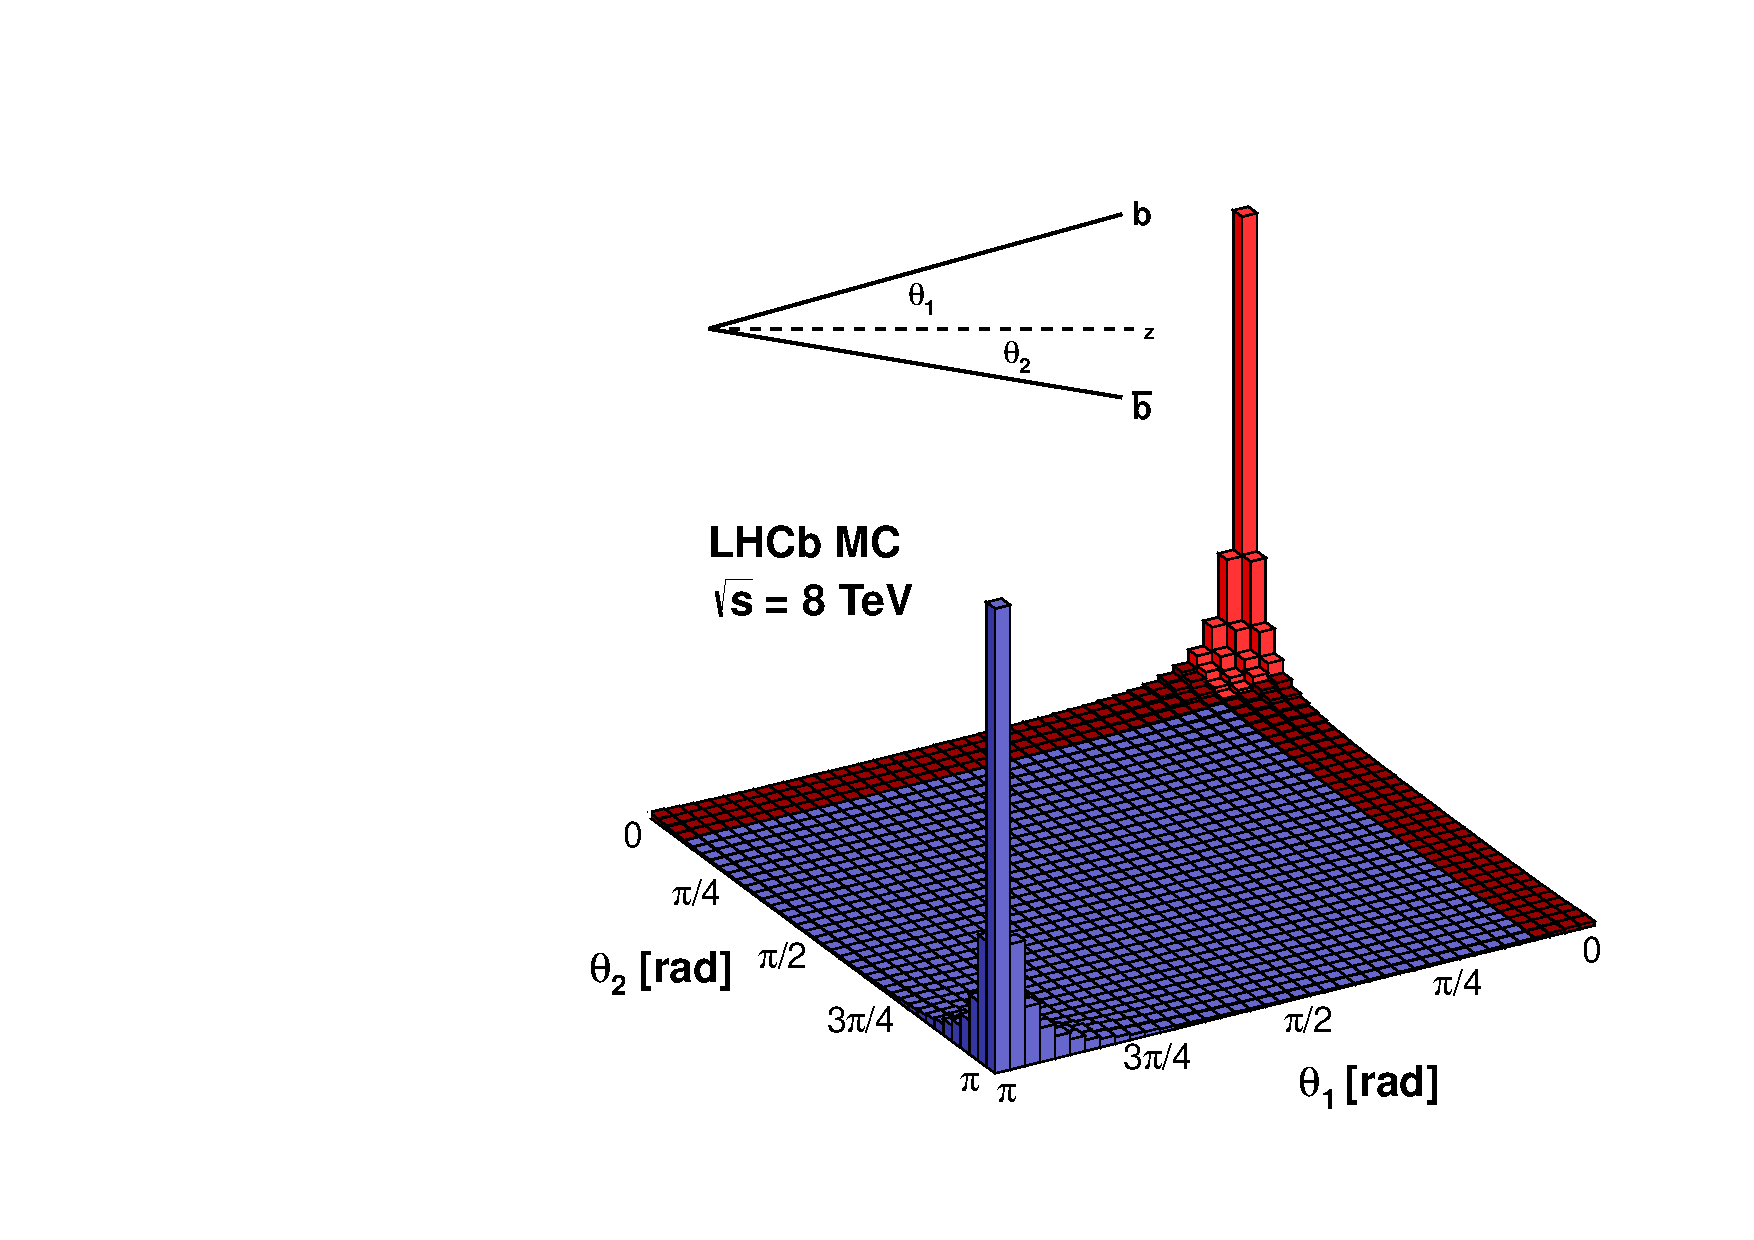
\includegraphics[width=0.5\textwidth]{08_rad_acc_scheme_right.pdf}
  \caption{A diagram showing the angular distribution of $b \bar{b}$ pair production at 8TeV}
  \label{fig:bbarprod}
\end{figure}
\subsection{Tracking}
\label{sec:Tracking}
The objective of any particle physics tracking system is to provide positional information on the path taken by chraged particles.  At all collider based experiments the paths of charged particles are curved by a magentic field to distinguish positive and negatively charged particles and also aid particle identification.  At \lhcb this is performed by a warm dipole magnet, which is subject to a polarity reversal periodically to remove systematic uncertainties.

The first stage of the \lhcb tracking system is the Vertex Locator (VELO).  When a \Bd meson is created it will travel a measurable distance before it decays.  As the \Bd is neutral it leaves no track, therefore there is a secondary or displaced vertex present in the decay.  This is also the case for many other mesons containing b and c quarks.  As these make up such a large section of the \lhcb phyiscs programme the VELO was developed to detect these secondary vertices.

The VELO consists of several circular silicon sensors which are placed transverse to the beam pipe, with the beam pipe passing through the center.  A diagram of this is shown in Figure \ref{fig:VELO}.  As shown in Figure \ref{fig:detectdiag} these are positioned before any other detector component as close as possible to the interaction region.  There are two types of sensors, one which provides radial position information of tracks and one which provides azimuthal $(\phi)$ position information.  These work in tandem to provide an optimal track resolution of $4\mu m$ \cite{Aaij:1978280}, which is the best of any tracking system at the LHC.
\begin{figure}
  \centering
  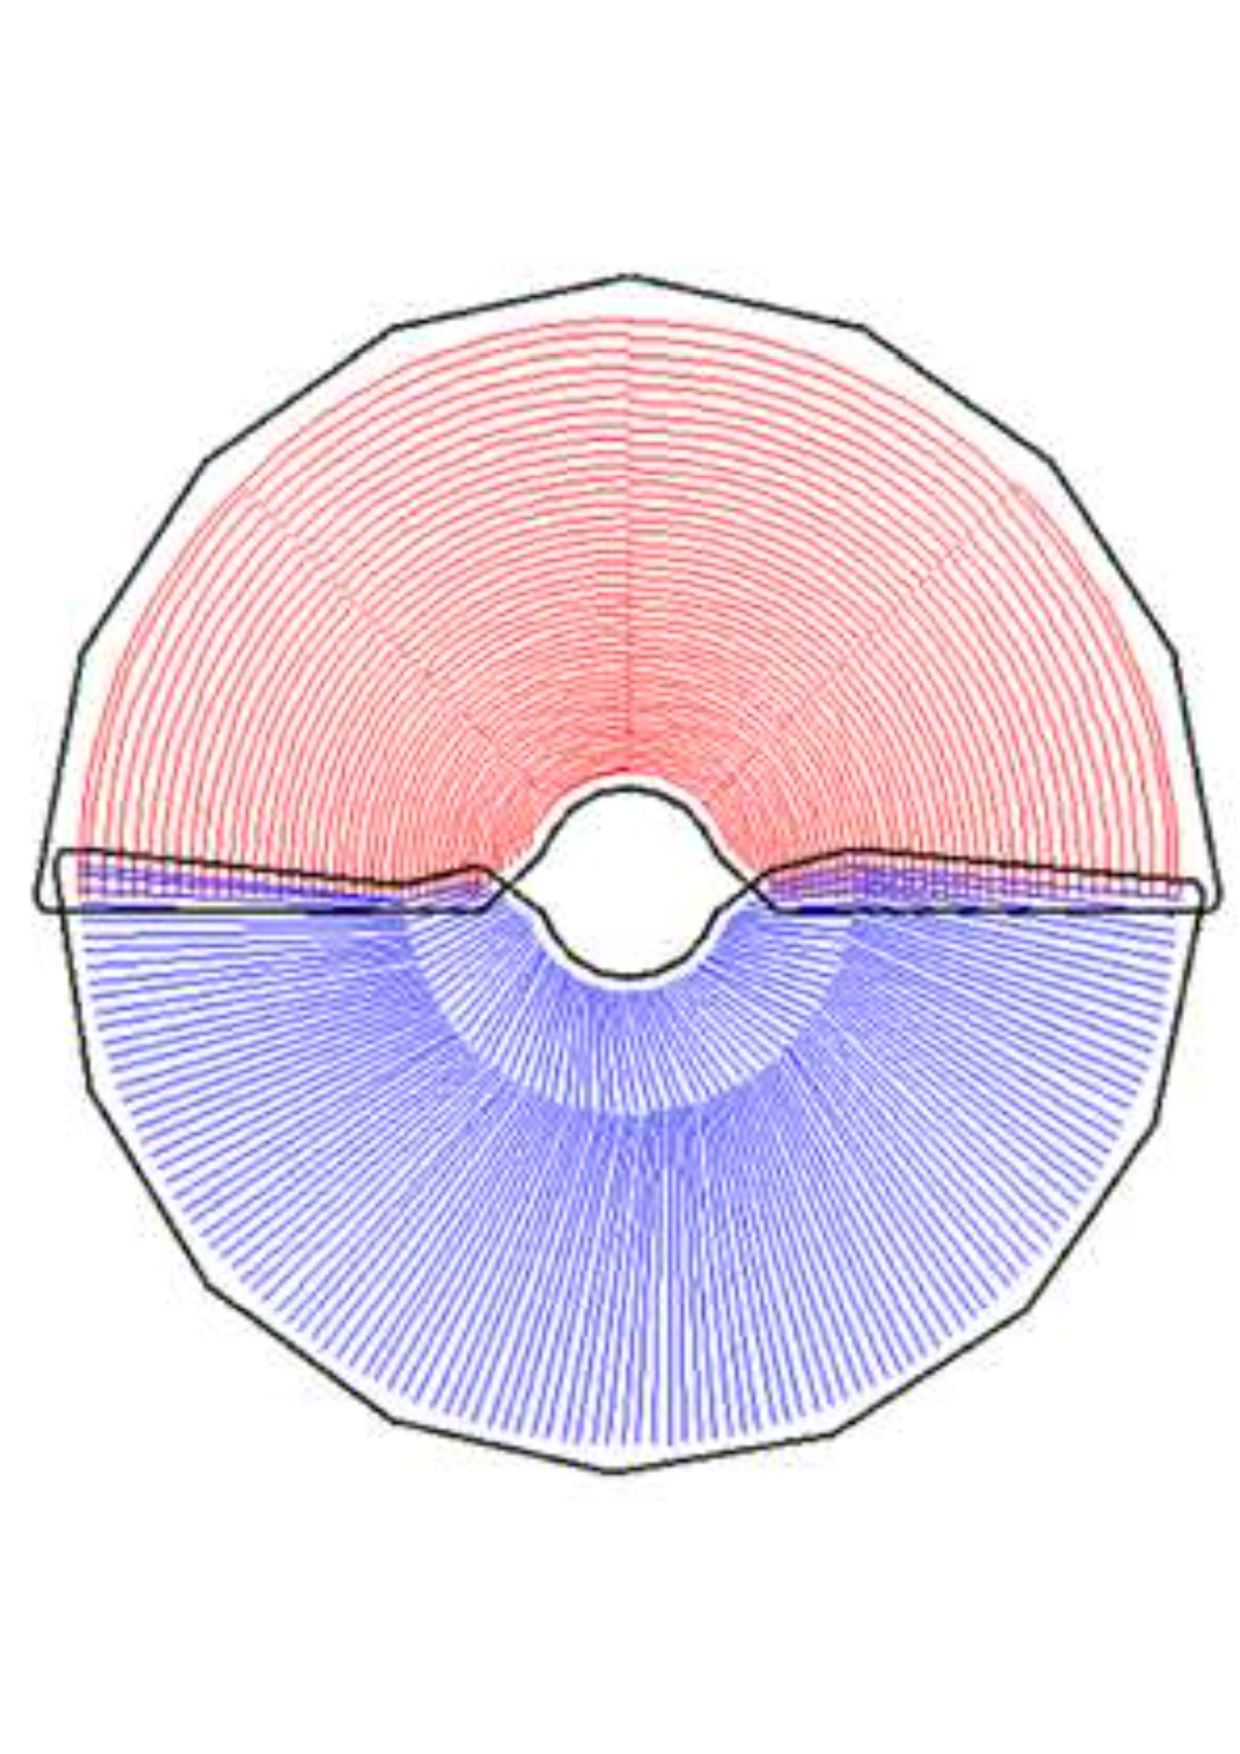
\includegraphics[width=0.5\textwidth]{VELO.pdf}
  \caption{A diagram showing half of each type of VELO sensor in the x,y plance.  The blue sensor provides azimuthal position information and the red sensor provides radial position information.}
  \label{fig:VELO}
\end{figure}

 In one year of running the VELO receives a 1MeV neutron equivalent fluence of $1.3\times10^{14} neq/cm^2$ which makes radiation hardness a challenge \cite{Alves:1129809}.  To keep this fluence to a minimum, the VELO is mechanically moved further away from the beam pipe whilst the LHC is still filling.  During this stage no physics data can be taken, therefore the VELO would be undergoing irrdation for no gain in physics data.

 The next stage of the \lhcb tracking system is positioned just upstream of the dipole magnet, denoted ``TT'' in Figure \ref{fig:detectdiag}.  This also makes use of silicon microstrips to give a positional resolution of $52.6 \mu m$, as measured in run I data \cite{Aaij:1978280}.

The final stage of the tracking system is positioned downstream of the dipole magnet, which is actually 3 seperate tracking stations labelled T1,T2 and T3 in Figure \ref{fig:detectdiag}.  The inner areas of these tracking stations are silicon microstrips which provide very similar spatial resolution to the TT.  As silicon microstrips are very expensive, the outer areas of the downstream tracking stations are straw tube trackers.  These provide a spatial resolution of $205 \mu m$ \cite{Aaij:1978280}.

 
\subsection{Calorimetry}
\label{sec:Calorimetry}
The role of calorimetry in HEP experiments is predominantly to measure the energy of particles.  However they also play a role in particle identification and, particularly at the LHC, a role in triggering.

The electromagentic calorimeter used by \lhcb is a tried and tested shashlik sampling calorimeter.  It consists of 66 seperate layers, each consisting of 2mm of lead and 4mm of plastic scintillator.  This amounts to 25 radiation lengths of material.  The role of the lead is to induce an electromagnetic shower as quickly as possible within short spatial constraints and the role of the scintillator is to measure the energy contained in the EM shower.

The light from the plastic scintillator is transported to photo multiplier tubes by wavelength shifting fibres.  These change the wavelength of the light from the plastic scintillator to a wavelength compatible with the photo multiplier tubes.  The signal from the PMTs is then proportional to the energy of the incident particle.

\subsection{Particle Identification}
\label{sec:Particle Identification}


%Muons

\clearpage
